\skriptsection{Description and Representation (V10, 11, 12)}{795}
  \skriptsubsection{Representation}{796}
    A region can be represented in terms of its external characteristics (its boundary - basically for shape properties) or
    its internal characteristics (pixels comprising the region - basically for regional properties (colors, texture)).
    
    Description is the extraction of information out of the representation. For example the length
    of a boundary.
    
    These are some basic methods: Chain Codes \formelbuch{798}, Polygonal Approximations 
    \formelbuch{801} and Skeletons \formelbuch{812}.
    
    \begin{tabular}{ll}
      \parbox{10cm}{
        \skriptsubsubsection{Signatures}{808}
          Signature: 1d representation of a boundary that can be generated in various ways.
          
          Example: Distance from the centroid to the boundary as a function of angle:\\
          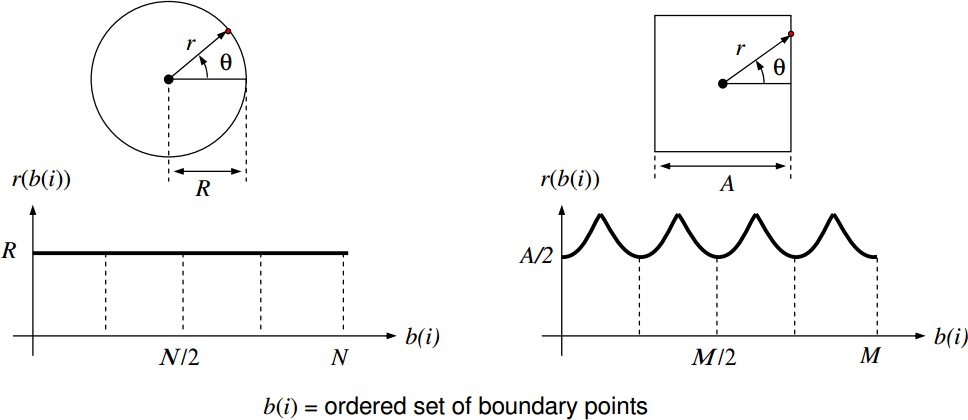
\includegraphics[width=9cm]{./images/signature.png}
          
          This signature generation is translation variant but not rotation or scaling variant.
          
          Features that can be used further are e.g. the number of maxima or the distance between maximum and minimum.}
      & \parbox{9cm}{
          \skriptsubsubsection{Fourier Descriptors}{818}
            FDs represent the frequency content of a shape (of the border) which can also be viewed as the form of an object.
            It is possible to make them independent of various transformations:\\
            \begin{tabular}{ll}
              Translation & $F(0) = 0$\\
              Scale & $F(u) = \frac{F(u)}{|F(1)|}$\\
              Rotation, starting point , direction & $F(u) = |F(u)|$ 
            \end{tabular}
            FDs are insensitive to noise.
            
            However, this might be dangerous as information (phase) is thrown away and may lead to wrong assumptions:\\
            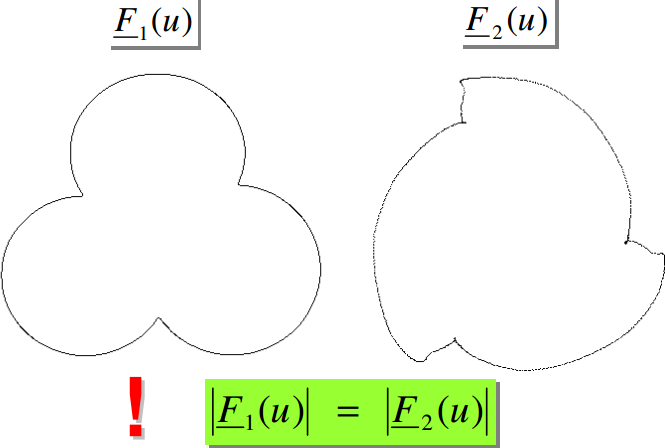
\includegraphics[width=5cm]{./images/fourier_descriptiors_danger.png}
            }
    \end{tabular}
      
      
    
    \skriptsubsubsection{Hough Transform (HT)}{735}
      Aim: Find lines, circles or any freeform shapes in an image after edge detection.
      
      \subsubsubsection{HT for Lines}
      The objects are found using the following algorithm:\\
      \begin{tabular}{|l|l|}
        \hline
        \textbf{Step} & \textbf{Example: Line} \\
        \hline
        Define mathematical equation which describes the shape.
          & $y = a_k x + b_k$ \\
        \hline
        Define parameter space with limits
          & $a_k \in [a_{min}, a_{max}]$, $b_k \in [b_{min}, b_{max}]$ \\
        \hline
        \parbox{9cm}{For every point $x_i$, $y_i$ solve $b = y_i-ax_i$ and increment each visited 
          point: $H(a,b)=H(a,b)+1$ \todo{check}}
          & \parbox{9cm}{
            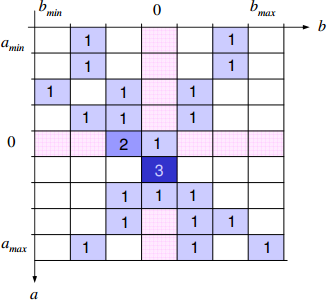
\includegraphics[width=6cm]{./images/hough_transform_parameterspace.png}
            } \\
        \hline
        Find maximum value in parameter space
          & Marked deep blue in graphics above (with 3 in it) \\
        \hline
        Parameters inserted into equation leads to most likely object
          & $y = a x + b$ \\
        \hline
      \end{tabular}
      
      Problem with this is that a horizontal line leads to $a \rightarrow \infty$. Therefore,
      the parameter equation $x \cos(\Theta) +  \sin(\Theta) = r$ should be used for finding
      a line.
      
      \subsubsubsection{Equations for circles}\\
      \begin{tabular}{lll}
        \parbox{8cm}{Cartesian equation:\\
           $r^2 = (x-x_0)^2 + (y-y_0)^2$ \\ \\
           Parametric representation:\\
           $x=x_0 + r \cos(\Theta)$\\
           $y=y_0+r\cos(\Theta)$\\
           with $\Theta$ not being a free parameter}
          & \parbox{5cm}{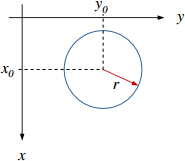
\includegraphics[width=4cm]{./images/hough_transform_circle.png}}
          & \parbox{5cm}{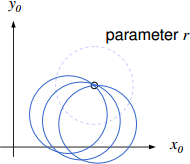
\includegraphics[width=4cm]{./images/hough_transform_circle2.png}}
      \end{tabular}
      
      
      \subsubsubsection{Generalized Hough Transform (GHT)}\\
        For freeform shapes which are rotation and scaling invariant as well as some a priori 
        knowledge of the shape is available.
        Here, the \em gradient of the boundary \em is used instead of a parameter model. The space is now called \em reference
        space \em and not parameter space anymore.
        
      \subsubsubsection{Conclusions}
        \begin{liste}
        	\item Quite high computational effort (``Brute Force''), but control by quantization of parameter space
        	\item Multiple objects can be detected
        	\item HT tolerates also objects with ``holes'' 
        \end{liste}
    
    \subsubsection{Harris Corner Detection}
      \begin{tabular}{ll}
        \parbox{13cm}{
          Corners are reference landmarks in images and help in localization.
          A corner has two large eigenvalues in the structure tensor $T_s$.
          
          \begin{aufzaehlung}
            \item  if necessary (eg. noise, etc.) low-pass filter the image 
            \item  compute gradients $G_x$, $G_y$ (sobel)
            \item  build the structure tensor: 4 (3) values per pixel
            \item  low-pass filter each component of the structure tensor
            \item  compute Harris corner measure $R(x,y)$ from structure tensor
            \item  threshold $R(x,y)$ with $T_th > 0 \rightarrow$ potential corners
            \item  use non-maxima suppression to find maxima in $R(x,y)$
              \begin{liste}
                \item sort maxima in descending order
                \item select largest maximum
                \item suppress maxima within radius $r$ around selected maximum
                \item select remaining largest maximum
                \item ... etc
              \end{liste}
          \end{aufzaehlung}
          }
          & \parbox{5cm}{
            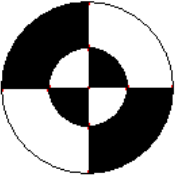
\includegraphics[width=4cm]{./images/marker.png}}
      \end{tabular}
      

  \clearpage
  \begin{minipage}{9cm}
  \skriptsubsection{Simple Descriptors}{822}
    Simple descriptors include area, perimeter, minimum/maximum diameter, area of bounding rectangle and
    should be independent of translation, rotation and scale.
     
    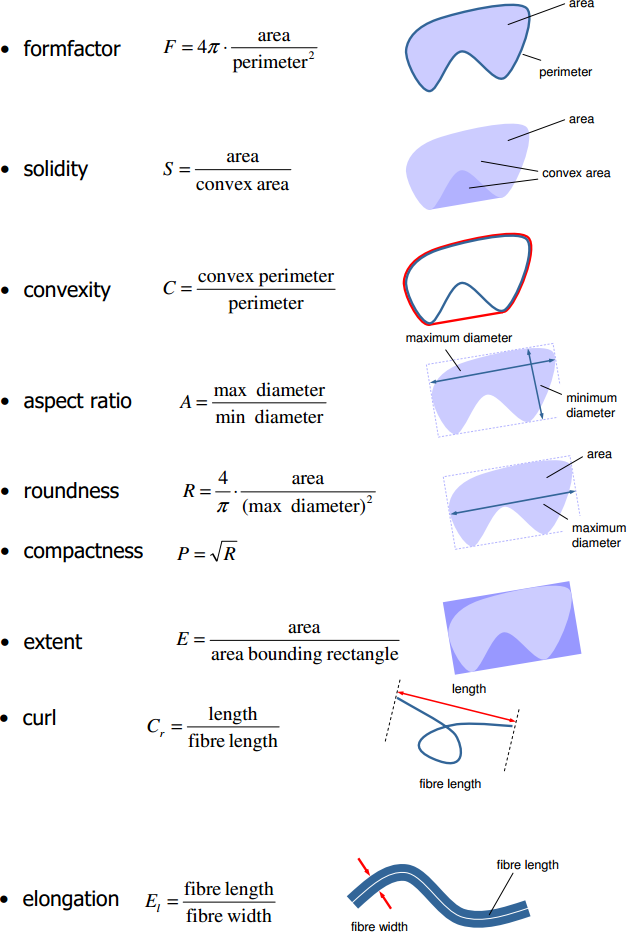
\includegraphics[width=8cm]{./images/simple_descriptors.png}
    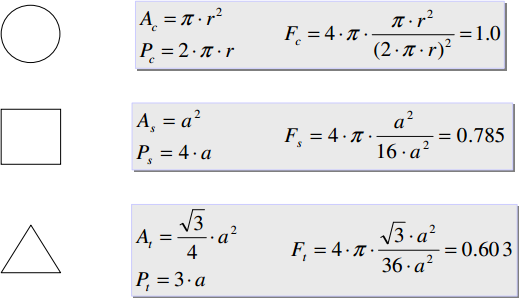
\includegraphics[width=8cm]{./images/simple_descriptors_formfactors.png}
    
    
    \skriptsubsection{Area Based Descriptors (Moments)}{839}
      Moments are statistical measures of the shape of a set of points. Due to its statistical
      nature, they are hardly variant to translation, rotation and scale.
      
      2D moments of order $p+q$: $$m_{pq} = \sum_{x=0}^{M-1} \sum_{y=0}^{N-1} x^p y^q f(x,y)$$
      
  \end{minipage}
  \begin{minipage}{9cm}
    \textbf{Area based descriptors, continued}
    
      2D \em central \em moments of order $p+q$: $$\mu_{pq} = \sum_{x=0}^{M-1} \sum_{y=0}^{N-1} (x-\bar{x})^p (y-\bar{y})^q f(x,y)$$
      with $\bar{x}=\frac{m_{10}}{m_{00}}$ and $\bar{y}=\frac{m_{01}}{m_{00}}$ which are also the
      centroid coordinates.
      
      Use principal components for normalizing with respect to variations in size, translation and 
      rotation.
      
      Moments provide:
      \begin{compactList}
        \item Centroid coordinates
        \item Principal axes of inertia (Trägheit) or direction of maximal and minimal 
          variance (principal components)
        \item Minimal bounding box
      \end{compactList}
    
    \skriptsubsection{Texture Based Descriptors}{827}
      \subsubsection{Statistical Approaches}
        Based on normalized histogram $h(g)$ (global):\\ 
        \begin{compactList}
          \item Mean: $m=\sum_{i=0}^{L-1} g_i h(g_i)$
          \item Variance: $\mu_2 = \sigma^2 = \sum_{i=0}^{L-1} (g_i-m)^2 h(g_i)$
          \item Skewness: $\mu_3 = \sum_{i=0}^{L-1} (g_i-m)^3 h(g_i)$
          \item Roughness: $R(g) = 1 - \frac{1}{1 + \sigma^2/(L-1)^2}$\\
            $R \rightarrow 1$: large $\sigma$, rough; $R \rightarrow 0$: $\sigma = 0$, smooth
          \item Uniformity (uniformity): $U(g) = \sum_{i=0}^{L-1} h^2(g_i)$
          \item Average entropy: \\$H(g) = -\sum_{i=0}^{L-1} h(g_i) \log_2(h(g_i))$
        \end{compactList}
      
      \subsubsection{Co-Occurence Matrix}
        The construction of COO uses the following scheme, it is local: \\
        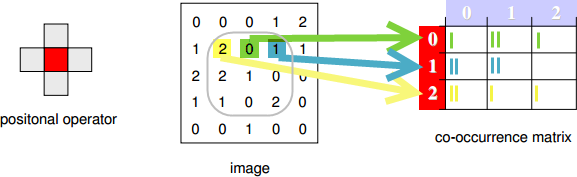
\includegraphics[width=8cm]{./images/cooccurence_matrix.png} \\
        The row index indicates the value of the center
        and the columns the number of values in the PO.
        
        The COO can also be reduced (instead of 255 grey intensities only 64 or 8 could be evaluated).
        
        \begin{tabular}{ll}
          Energy
            & $E = \sum_{i=0}^{L-1} \sum_{j=0}^{L-1} COO(i,j)^2$ \\
          Contrast
            & $C = \sum_{i=0}^{L-1} \sum_{j=0}^{L-1} (i-j)^2 COO(i,j)$ \\
          Entropy
            & $H = \sum_{i=0}^{L-1} \sum_{j=0}^{L-1} COO(i,j) \log(COO(i,j))$ \\
          Homogenity
            & $S = \sum_{i=0}^{L-1} \sum_{j=0}^{L-1} \frac{COO(i,j)}{1+|i-j|}$ \\
        \end{tabular}
        
    \subsubsection{Spectral Approach}
      Energy, contrast, entropy can also be found out using the scaled spectrum:
      $$S(u,v) = FFT(f(x,y)) \qquad S_n(u,v) = \frac{|S(u,v)}{\sqrt{\sum\limits_{u=2}^{m} \sum\limits_{v=2}^n |S(u,v)|}}$$
  \end{minipage}
    
    